\section{Characteristic energy for launch}

The characteristic energy for launch is the energy required to set a spacecraft
into the desired targeting orbit. This analysis assumes that the spacecraft
launches from Earth, which is modeled as a point with no mass and arrives at the
target interloper, modeled again as a massless point. The only force acting on
the spacecraft is the gravitational force of the Sun.

Before launching, the spacecraft has the velocity of Earth, $\vec{v_{\oplus}}$.
At launch, the spacecraft presents the velocity $\vec{v_1}$ that matches the
solution of Lambert's problem. Vector $\Delta{\vec{v}}$ is the difference
between the two velocities, and its modulus matches the required impulse
velocity, as stated in Equation \ref{eq:launch_velocity}.

\begin{equation}
    \Delta v_1 = \|\vec{v_1} - \vec{v_{\oplus}}\|
    \label{eq:launch_velocity}
\end{equation}

The value of $\Delta v_1$ can be used in Equation \ref{eq:c3} for solving the
characteristic for launch.

\subsection{'Oumuamua}

Porkchop plots for 'Oumuamua representing the characteristic energy for launch
are shown in figure \ref{fig:oumuamua-direct-prograde-transfer-porkchop} and
figure \ref{fig:oumuamua-direct-retrograde-transfer-porkchop}.

\begin{figure}[H]
  \centering
  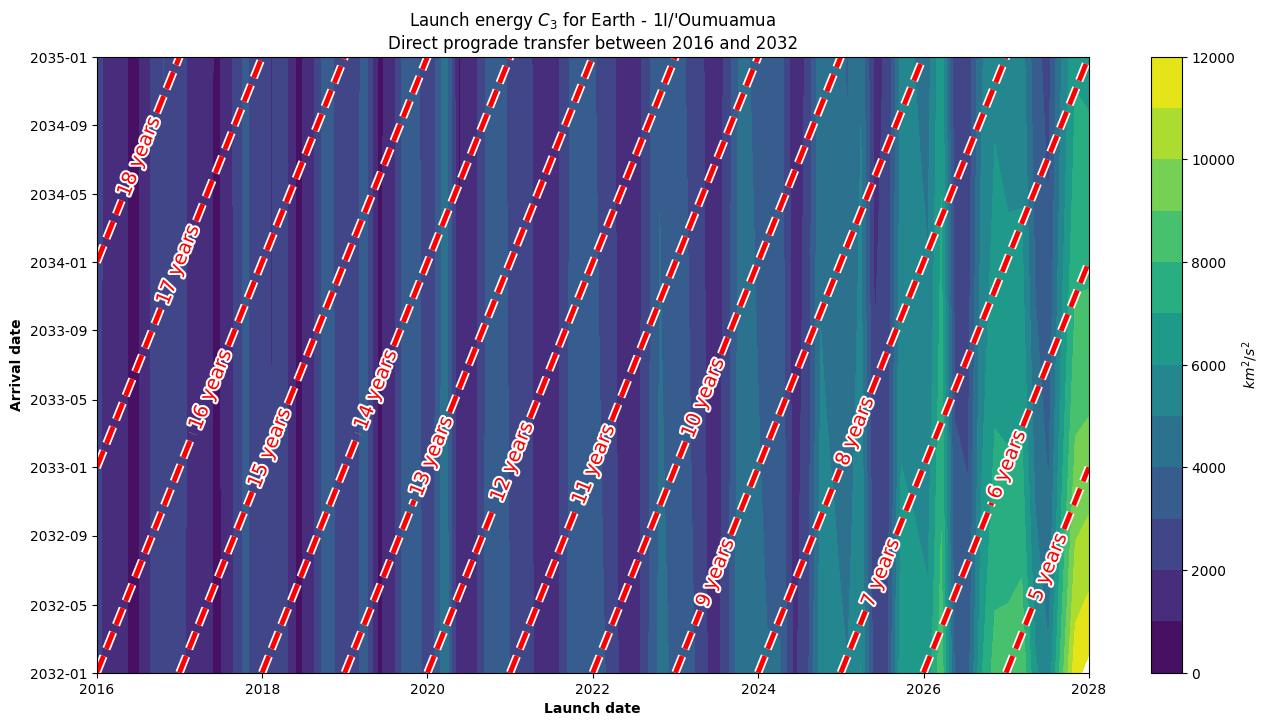
\includegraphics[width=\textwidth]{static/oumuamua/direct-prograde-transfer-porkchop.png}
        \caption[Direct and prograde launch energy porkchop for 'Oumuamua]{Launch energy porkchop plot for 1I/'Oumuamua for a direct and prograde
        transfer showing the isolines for
        the time of flight required for a targeting.}
  \label{fig:oumuamua-direct-prograde-transfer-porkchop}
\end{figure}

\begin{figure}[H]
  \centering
  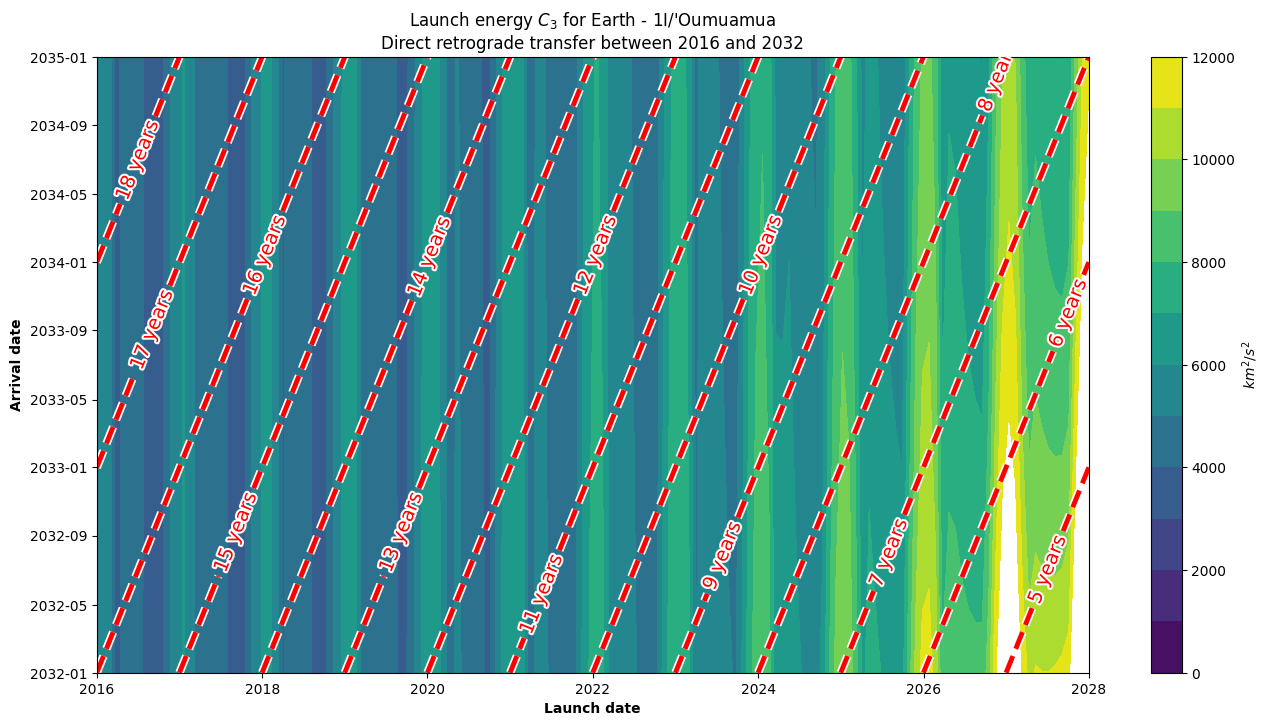
\includegraphics[width=\textwidth]{static/oumuamua/direct-retrograde-transfer-porkchop.png}
        \caption[Direct and retrograde launch energy porkchop for
        'Oumuamua]{Launch energy porkchop plot for 1I/'Oumuamua for a direct and
        retrograde transfer showing the isolines for
        the time of flight required for a targeting.}
  \label{fig:oumuamua-direct-retrograde-transfer-porkchop}
\end{figure}





\subsection{Borisov}

TODO
